\documentclass{book}
\usepackage{graphicx}
\usepackage[english]{babel}
\usepackage{amsthm}
\usepackage{amssymb}
\usepackage{amsfonts}
\usepackage{mdframed}
\usepackage{physics}
\usepackage{tikz}
\usepackage[a4paper, margin=1in]{geometry}
\geometry{a4paper, margin=1in}
\usepackage{xcolor}
\usetikzlibrary{arrows.meta}
\usetikzlibrary{angles,quotes}
\graphicspath{ {./images/} }
\usepackage{svg}
\usepackage{subcaption}
\usepackage{bm}
\usepackage{empheq}
\usepackage{cancel}
\usetikzlibrary{decorations.text}
\usepackage[most]{tcolorbox}
\usepackage{tensor}
%3D
\usepackage{mathtools}
\usepackage{booktabs}
\usepackage{array}
\newcolumntype{C}{>{$}c<{$}}
\usepackage{tikz-3dplot}
\usepackage{appendix}
\usepackage{pgfplots}
\usetikzlibrary{shapes.geometric}
\usetikzlibrary{calc,patterns,angles,quotes}
%Tikz Library
\usetikzlibrary{angles, quotes, intersections}
\usepackage[bb=dsserif]{mathalpha}
\usetikzlibrary{decorations.pathmorphing}
\usetikzlibrary {patterns,patterns.meta} 
\tikzset{snake it/.style={decorate, decoration=snake}}

\usepackage{etoolbox} % ifthen
\usepackage[outline]{contour} % glow around text
\usetikzlibrary{calc} % for adding up coordinates
\usetikzlibrary{decorations.markings,decorations.pathmorphing}
\usetikzlibrary{angles,quotes} % for pic (angle labels)
\usetikzlibrary{arrows.meta} % for arrow size
\usepackage{xfp} % higher precision (16 digits?)

\usepackage{tcolorbox}

%https://osl.ugr.es/CTAN/macros/latex/contrib/tcolorbox/tcolorbox.pdf
\tcbuselibrary{breakable}
\tcbset{%any default parameters
	width=0.7\textwidth,
	halign=justify,
	center,
	breakable,
	colback=white    
}

\newenvironment{aside}
{\begin{mdframed}[style=0,%
		leftline=false,rightline=false,leftmargin=2em,rightmargin=2em,%
		innerleftmargin=0pt,innerrightmargin=0pt,linewidth=0.75pt,%
		skipabove=7pt,skipbelow=7pt]\small}
	{\end{mdframed}}

\renewcommand{\cleardoublepage}{\clearpage}

\title{Electromagnetism 2}
\author{Dominik Szablonski}
\newtheorem{law}{Law}
\newtheorem{klaw}{Law}
\newtheorem*{definition}{Definition}
\newtheorem*{theorem}{Theorem}

\pgfplotsset{compat=1.18}
\begin{document}
\maketitle

\tableofcontents

\chapter{Sources of Radiation}
Radiation is the phenomenon of energy being transported to an observer. Radiation must be disconnected from its source. Plane electromagnetic waves satisfy conditions of being radiation, and are thus known as free fields. The source of electromagnetic radiation must be charges as those generate the electric and magnetic fields. However, electromagnetic radiation is only generated through accelerating charges. For a free field, there must be locations where radiation propagates while $\rho = 0$.
\section{Charges}
\subsection{Stationary Charges}
For a stationary charge, we can write,
\begin{align}
	\vb{E} = \frac{1}{4\pi\varepsilon_0}\frac{q(\vb{r} - \vb{r}')}{|\vb{r} - \vb{r}'|^3} \propto \frac{1}{|\vb{r} - \vb{r}'|^2} && \vb{B} & = 0
\end{align}
We can clearly see that a stationary charge cannot radiate as it has no component in $\vb{b}$. Furthermore, the energy flow varies as $\vb{1}{r^2}$, which require $\vb{E}\propto\frac{1}{r}$ and $\vb{B}\propto\frac{1}{r}$ which neither field satisfies.
\subsection{Charges with Uniform Velocity}
We can perform a Lorentz boost in the case of a moving charge,
\begin{equation}
	\vb{E}(\vb{r}) = \frac{q}{4\pi \varepsilon_0}\frac{1-\beta^2}{(1 - \beta^2\sin^2\theta)}\frac{\vu{r}}{|\vb{r}|^2}.
\end{equation}
We find that the electric flux still varies as $\frac{1}{r^2}$, thus cannot . Furthermore, we can move into the charge's rest frame where it still varies as $\frac{1}{r^2}$. This is the case as charge is both a conserved and Lorentz invariant quantity.
\\\\
We could also make the an argument using the Biot-Savarte law,
\begin{equation}
	\vb{B}(\vb{r}) = \frac{\mu_0}{4\pi}\frac{q\vb{v}\cross\vu{r}}{\left|\vb{r}\right|^2}
\end{equation}
which still varies as $\frac{1}{r^2}$. Thus, we require acceleration of the charge for radiation to occur.
\begin{aside}
	The reason we require that the electric field and magnetic field be proportional to $1/r$ is because of energy conservation. Let us recall that
	\begin{equation}
		\vb{S} = \frac{1}{\mu_0}\vb{E}\cross\vb{B}
	\end{equation}
	thus $S \propto EB$. We require,
	\begin{equation}
		\int S\cdot\dd{\vb{A}} = \text{Constant}
	\end{equation}
	for energy conservation. Since $\dd{A} \propto r^2$, we require $S \propto 1/r^2$, and thus $E,B \propto 1/r$.
\end{aside}
\section{Retarded Potentials}
If we recall eqs. \eqref{eq:A} and \eqref{eq:phi} of the sourced potentials, we can analyse more closely the static and dynamic cases to gain more insight into radiation phenomena.
\subsection{Statics}
In the static case, we clearly see that we recover Poisson's equation, which we can solve trivially.
\subsection{Time-Dependent case}
In the time dependent case, we require that the electric field propagates at the speed of light $c$. Thus, we wish to obtain a scalar potential $\phi(\vb{r},t)$ sue to a volume of charge $\rho\dd{V}'$ at $\vb{r}'$. We must use the charge density which existed in that volume at an earlier time $\tau$,
\begin{equation}
	\tau = t - \frac{|\vb{r} - \vb{r}'|}{c}
\end{equation}
where $\frac{|\vb{r} - \vb{r}'|}{c}$ is the time taken for information ot travel from $\vb{r}'$ to $\vb{r}$. We can call $\tau$ the \textit{retarded time}. We can thus write down the retarded potentials,
\begin{align}
	&\phi(\vb{r},t) = \frac{1}{4\pi\varepsilon_0}\int_V \frac{\rho(\vb{r}', \tau)}{|\vb{r} - \vb{r}'|}\dd{V}' \\
	&\vb{A}(\vb{r},t) = \frac{\mu_0}{4\pi}\int_V\frac{\vb{J}(\vb{r}',\tau)}{|\vb{r}- \vb{r}'|}\dd{V}'
\end{align}

\section{Radiation from an accelerated charge}
\subsection{Displaced point charge}
\begin{figure}
	\centering
	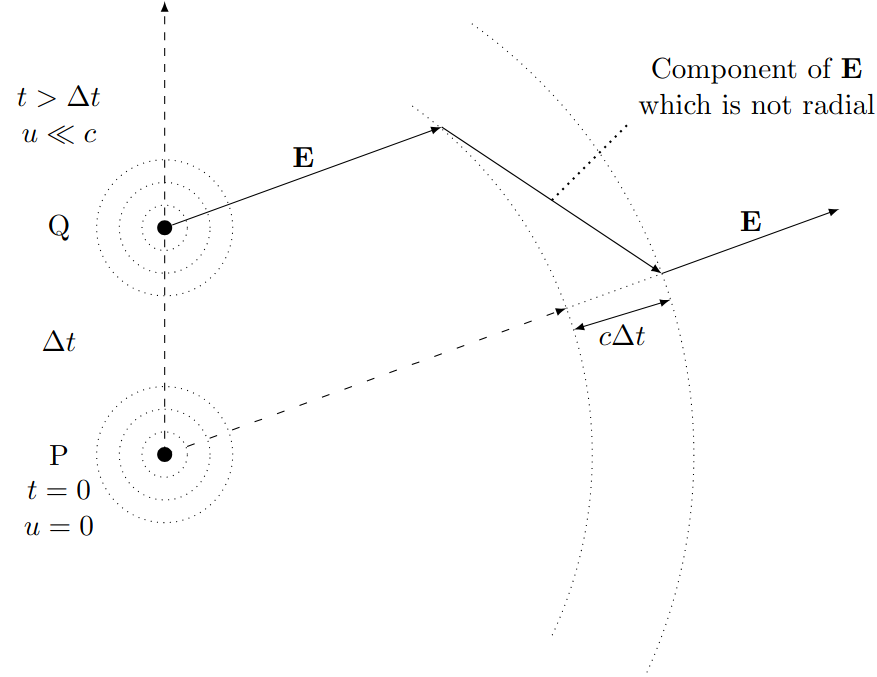
\includegraphics[width=0.75\textwidth]{2.3.png}
	\caption{}
	\label{fig:2.3}
\end{figure}
Consider figure \ref{fig:2.3}, initially at rest at point $P$ in free space. It is given a sudden impulse and undergoes a sudden acceleration $a$ over a short time $\Delta t$, such that when the charge reaches $Q$ it is moving at a constant velocity $u = a\Delta t << c$. If we consider the observer at a far away distance $r$, they will still see the charge at its original, stationary position. In order to see the charge move, the observer must wait a time $t = r/c$. In this time, there must be a boundary where the field configurations move from the old stationary state to the moving state. This boundary will have a width $c\Delta t$ and will must move away from the charge's location at a speed $c$.
\\\\
Let us recall that $\div{\vb{E}} = 0$, so there can be no discontinuities in the field lines generated by the charge. The boundary thus presents itself as a \textit{kink} in the electric field lines, as shown in figure \ref{fig:2.3}. This is a component of $\vb{E}$ which is not radial. 
\begin{figure}
	\centering
	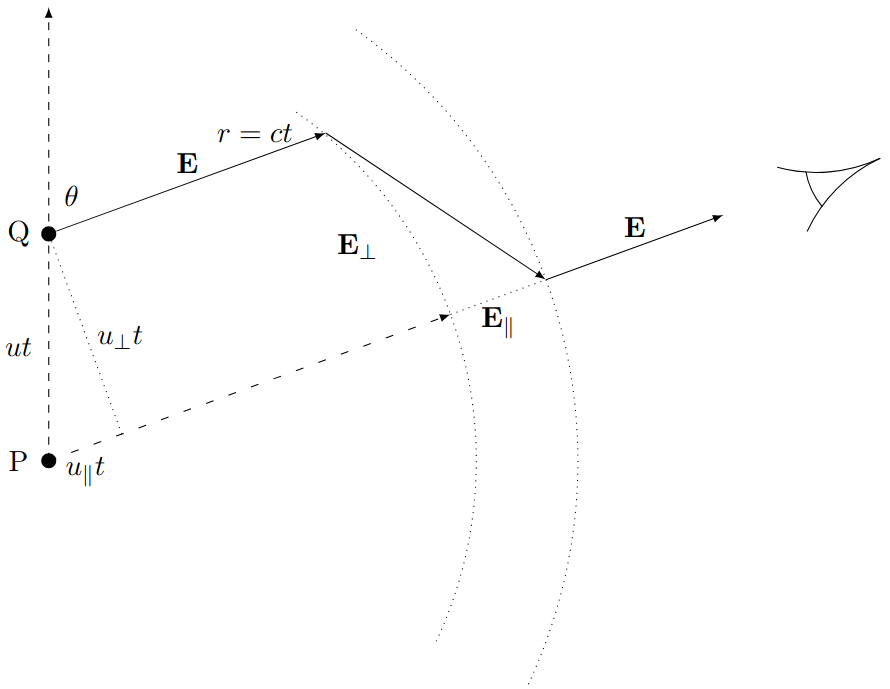
\includegraphics[width=0.75\textwidth]{2.4.png}
	\caption{}
	\label{fig:2.4}
\end{figure}
\\\\
Let us now consider the observer looking at the charge at some angle $\theta$ while it undergoes its final motion, reaching a position $ut$. Let us note that the boundary of observing the charge's motion is
\begin{equation}
	r = ct.
\end{equation}
According to the observer, the charge appears at $u_{\parallel}t$ parallel to their line of sight and  $u_{\perp}t$ perpendicular to their line of sight. We can then relate these to the parallel and perpendicular components of the kink $E_{\parallel}$ and $E_{\perp}$,
\begin{equation}
	\frac{E_{\perp}}{E_{\parallel}} = \frac{u_{\perp} t}{c\Delta t}.
\end{equation}  
If we note that $u_{\perp} = a_{\perp}\Delta t$, we can write,
\begin{equation}
	E_{\perp} = E_{\parallel}\frac{a_{\perp}r}{c^2}.
\end{equation}
Furthermore, since the charge's field is radial, we can say,
\begin{equation}
	E_{\parallel} = \frac{1}{4\pi\varepsilon_0}\frac{q}{r^2}
\end{equation}
so we can write,
\begin{equation}
	E_{\perp} = \frac{1}{4\pi\varepsilon_0}\frac{qa_{\perp}}{c^2r}.
\end{equation}
Let us summarise what we have found using this thought experiment,
\begin{enumerate}
	\item The field $E_{\perp} \propto 1/r$ in the kink region.
	\item Recalling equation \eqref{eq:A4}, we see $B_{\perp} = E_{\perp}/c$ in the kink region.
	\item The magnitude of the Poynting vector $\vb{S} = \frac{1}{\mu_0}\vb{E}\cross\vb{B}$ is, $S \propto EB \propto 1/r^2$
\end{enumerate}
which satisfy our conditions for radiation.
\subsection{Radiation pattern from a displaced point charge}
We wish to now consider the electric field and the power flux (Poynting vector) as time dependent functions, noting that we will require using the retarded time. By noting that $a_{\perp} = a \sin\theta$, we can simply write,
\begin{equation}
	\abs{\vb{E}(\vb{r},t)} = \frac{1}{4\pi\varepsilon_0}\frac{q\abs{\vb{a}\left(t - \frac{r}{c}\right)}\sin\theta}{c^2r}.
\end{equation}
Then, we can write the Poynting vector as,
\begin{equation}
	\abs{\vb{S}(\vb{r},t)} = \frac{1}{16\pi^2\varepsilon_0}\frac{q^2\abs{\vb{a}^2\left(t - \frac{r}{c}\right)}\sin^2\theta}{c^3r^2}. \label{eq:poynt}
\end{equation}
\subsection{Total Power Radiated}
The Poynting vector is the directional energy flux per unit area, per unit time. Thus, to find the power radiated, we simply compute the integral,
\begin{equation}
	P(t) = \oint \vb{S}\cdot\dd{\vb{A}} = \int_0^{2\pi}\int_0^{\pi} S r^2\sin\theta \dd{\theta} \dd{\phi}.
\end{equation}
Substituting expression \eqref{eq:poynt}, we obtain Larmor's formula,
\begin{equation}
	\boxed{P(t) = \frac{q^2\left[a\left(t-\frac{r}{c}\right)\right]^2}{6\pi \varepsilon_0c^3}}.
\end{equation}
\section{Radiation from an Oscillating Electric Dipole}
\begin{figure}
	\centering
	\begin{tikzpicture}
		\draw[<->] (0,0) -- (0,4);
		\node at (0,1) {\textbullet};
		\node at (0,3) {\textbullet};
		\node[anchor=west] at(0,1) {$q$};
		\node[anchor=west] at(0,3){$q$};
		\draw [->] (0,2) -- (2,2);
		\draw [latex-latex] (-0.5,1) -- (-0.5,3) node[midway, anchor=east] {$l$};
	\end{tikzpicture}
	\caption{}
	\label{fig:dipole}
\end{figure}
Consider an oscillating dipole, with charges separated by a length $l$ and oscillating along the $z$ axis. From Larmor's formula, $P(t) \propto \left(qa(\tau)\right)^2$. We can approximate the oscillating charges as a charge distribution with charge per unit length $\mu$ and length $l$. We can write,
\begin{equation}
	\begin{split}
		qa(\tau) & = \mu la(\tau) \\
		& = \mu \dv{v}{\tau}l \\
		& = l \dv{(\mu v(\tau))}{\tau}
	\end{split}
\end{equation}
where we find $\mu v(\tau)$ to have units of current, i.e., $\left[\mu v(\tau)\right] = [A]$. We can represent this as a current,
\begin{equation}
	\mu v (\tau) =  I(\tau) = I_0\cos\omega t
\end{equation}
where $I_0$ and $\omega$ are the corresponding amplitude and angular frequency of oscillation. Thus, we can write $qa(\tau)$ as,
\begin{equation}
	qa(\tau) = - \omega L I_0 \sin(\omega t - kr).
\end{equation}
By substitution, we can find the corresponding electric and magnetic fields,
\begin{align}
	E_{\perp} = \frac{I_0 l \sin\theta}{4\pi \varepsilon_0 rc^2}\omega \sin(\omega t - kr) && B_{\perp} = \frac{I_0 l \sin\theta}{4\pi \varepsilon_0 rc^3}\omega \sin(\omega t - kr) \label{eq:hertzian}
\end{align}
and the corresponding power emitted is,
\begin{equation}
	P = \left[\frac{l^2 \omega ^2}{6\pi \varepsilon c^3}\right]I_0 \sin^2(\omega t - kr). \label{eq:powerrad}
\end{equation}
\subsection{Radiation Resistance}
If we recall the formula $P = I^2 R$, we find that we can extract a resistance from equation \eqref{eq:powerrad}. This is known as the \textit{radiation resistance}, given by,
\begin{equation}
	R_{\text{rad}} = \frac{l^2 \omega ^2}{6\pi \varepsilon c^3}
\end{equation}
\section{Half-Wave Antenna}
\begin{figure}
	\centering
	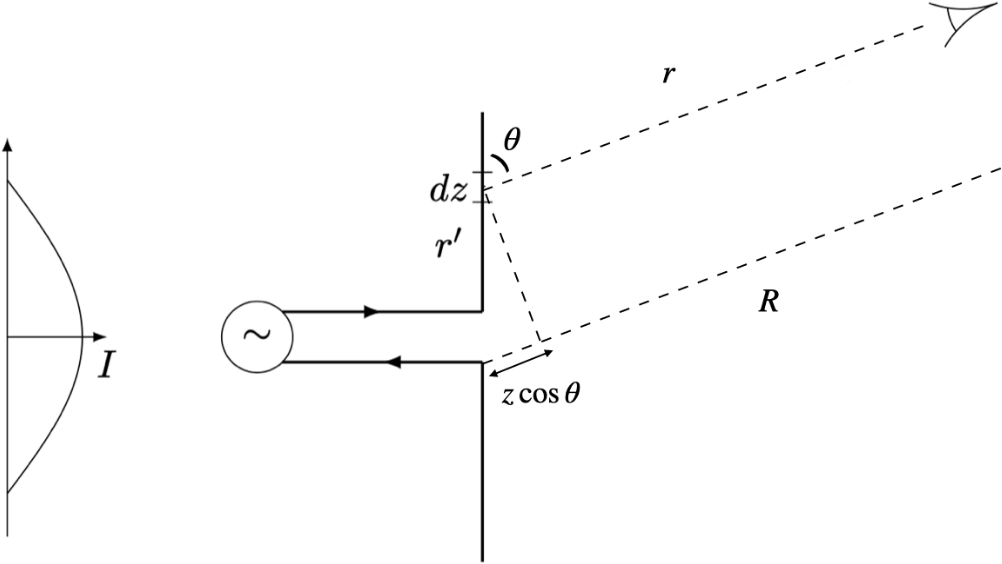
\includegraphics[width=0.5\textwidth]{2.6.png}
	\caption{}
	\label{fig:2.6}
\end{figure}
Let us consider a more realistic antenna, as in figure \ref{fig:2.6}. This is a centre fed, thin, straight antenna of length $l$. The solution for the current distribution of this antenna can be obtained from Maxwell's equations, whose solution is,
\begin{equation}
	I(z) = I_0 \sin\left(m\pi \left(\frac{\abs{z}}{l} + \frac{1}{2}\right)\right)
\end{equation}
where $m$ is an integer. We can integrate the Hertzian dipole over the length of the antenna in order to obtain an expression for the electric field, we have
\begin{equation}
	\dd E = \frac{I(z) \dd{z}\sin\theta}{4\pi \epsilon_0 r c^2}\omega \sin(\omega t - kr).
\end{equation}
Before we integrate this, we must consider the phase $\omega t - kr$. We find that there will be a time-lag of $\Delta t \frac{z\cos\theta}{c}$, with a resultant lag in phase of $kz\cos\theta$. Furthermore, we can approximate $r \approx R - z\cos\theta$, thus our integral becomes,
\begin{equation}
	E = \frac{\omega \sin\theta}{4\pi \varepsilon_0Rc^2}\int_{-l/2}^{l/2}I(z) \sin\left(\omega t - kR + kz\cos\theta\right)\dd{z}
\end{equation}
and computing this,
\begin{equation}
	E = \frac{I_0 l}{4\pi \varepsilon_0Rc^2}\left[\frac{2}{\pi}\frac{\cos\left(\frac{\pi}{2}\cos\theta\right)}{\sin\theta}\right]\omega \sin\left(\omega t - kR\right).
\end{equation}
We wish to then find the time-averaged poynting vector, computed by $\langle S \rangle = \frac{1}{\mu_0}\langle \vb{E}\cross\vb{B}\rangle$, which we find to be,
\begin{equation}
	\langle S \rangle = \frac{I_0^2}{8\pi^2 \mu_0\varepsilon_0^2R^2c^3}\frac{\cos^2\left(\frac{\pi}{2}\cos\theta\right)}{\sin^2\theta}.
\end{equation}
We can then compute the time average of the power radiated by $\langle P \rangle = \oint \langle S \rangle\dd{A}$, which requires us to compute,
\begin{equation}
	\langle P \rangle = \frac{I_0^2}{4\pi \mu_0\varepsilon_0^2 R^2c^3}\int_0^{\pi}\frac{\cos^2\left(\frac{\pi}{2}\cos\theta\right)}{\sin\theta}\dd{\theta}
\end{equation}
We then find,
\begin{equation}
	\langle P \rangle \simeq 1.22\frac{I_0^2}{r\pi \varepsilon_0 c} \simeq 0.194Z_0I_{\text{rms}}^2
\end{equation}
where we define $Z_0 = \frac{1}{\varepsilon_0 c} = \sqrt{\frac{\mu_0}{\varepsilon}}$ and $I_{\text{rms}} = \frac{I_0^2}{2}$.

\chapter{Radiation in Matter}
\section{Maxwell's Equations in a Medium}
Let us recall electromagnetic fields in materials. 
\subsection{Electrics}
The $\vb{P}$ field is the dipole moment per unit volume, and describes bound charges, such that,
\begin{align}
	\div{\vb{P}} = \rho_b && \vb{P}\cdot\vu{n} = \sigma_b
\end{align}
where $_b$ indicates a bound charge, and $\sigma_b$ is the bound surface charge. The total charge is composed of bound charge and free charge, such that $\rho = \rho_b + \rho_f$. We can then define the $\vb{D}$ field, such that,
\begin{equation}
	\div{\vb{D}} = \rho_f
\end{equation} 
for linear dielectrics, and,
\begin{equation}
	\vb{D} = \epsilon_0\vb{E} + \vb{P} = \epsilon_0\epsilon_r\vb{E}
\end{equation}
where $\epsilon_r = 1 + \chi_E$.
\subsection{Magnetics}
In magnetics, materials can have different types of magnetism:
\begin{itemize}
	\item \textit{Paramagnetism:} Magnetisation parallel to $\vb{B}$, dipoles align with $\vb{H}$.
	\item \textit{Diamagnetism:} Magnetisation is antiparallel with $\vb{B}$, dipoles anti-align with $\vb{H}$.
	\item \textit{Ferromagnetism:} Magnetisation is retained even after $\vb{B}$ is removed, regions of dipoles align together with $\vb{H}$.
\end{itemize}
We can define the magnetisation $\vb{M}$ as the magnetic dipole moment per unit volume, from which we can obtain the bound and surface currents,
\begin{align}
	\vb{j}_b = \curl{\vb{M}} && \vb{K}_b = \vb{M} \times \vu{n}.
\end{align}
We can then define a $\vb{H}$ field for free currents such that,
\begin{equation}
	\curl{\vb{H}} = \vb{J}_f
\end{equation}
where,
\begin{equation}
	\vb{H} = \frac{1}{\mu_0}\vb{B} - \vb{M} = \frac{1}{\chi_M}\vb{M} = \frac{1}{\mu_0\mu_r}\vb{B}.
\end{equation}
\subsection{Time dependent case}
\begin{align}
	\div{\vb{D}} = \rho_f && \div{\vb{B}} = 0\\
	\curl{\vb{H}} = \pdv{\vb{D}}{t} + \vb{j}_f && \curl{\vb{E}} = -\pdv{\vb{B}}{t}
\end{align}
\section{Plane Waves in Lossy Media}
Consider electromagnetic waves travelling in the $z$ direction such that,
\begin{align}
	\vb{E} = \left(E_x, 0, 0\right) && E_x = E_0e^{i(\omega t - kz)} \\
	\vb{B} = \left(0, B_y, 0\right) && B_y = B_0e^{i(\omega t - kz)}
\end{align}
Considering Faraday's law, we get,
\begin{equation}
	-ikE_0e^{i(\omega t - kz)} = -i\omega B_0 e^{i(\omega t - kz)}
\end{equation}
and thus,
\begin{equation}
	\frac{B_0}{E_0} = \frac{k}{\omega}.
\end{equation}
Recalling Ohm's law $\vb{J} = \sigma \vb{E}$ where $\sigma$ is the conductivity, and Ampere's law, we obtain,
\begin{equation}
	k^2 = \frac{\omega^2}{c^2} \epsilon_r\mu_r - i\omega \mu_r\mu_0 \sigma \label{eq:dispersion} 
\end{equation}
which is the dispersion relation for a linear, isotropic, dielectric medium. We see that this expression is complex, and reduces to the vacuum condition under vacuum. 
\subsection{Source-Free Lossy Media}
Let us consider a conducting media with dielectric properties and free current $\vb{J}_f$. Using Ampere's law,
\begin{equation}
	\begin{split}
		\curl{\vb{H}} & = \pdv{\vb{D}}{t} + \vb{J}_f \\
		& = i \omega \epsilon_0\epsilon_r \vb{E} + \sigma \vb{E} \\
		& = (i\omega \epsilon_0\epsilon_r + \sigma)\vb{E} \\
		& = i\omega(\epsilon_0\epsilon_r + \frac{\sigma}{i\omega})\vb{E}.
	\end{split}
\end{equation}
We can then define the \textit{complex permittivity},
\begin{equation}
	\epsilon_c = \epsilon_0\epsilon_r - \frac{i\sigma}{\omega}
\end{equation}
which we apply to conducting media. In the case of complex media, Ampere's law becomes $\curl{\vb{H}} = i\omega\epsilon_c\vb{E}$, but otherwise, we simply replace $\epsilon_0\epsilon_r$ with $\epsilon_c$ to retrieve Maxwell's equations for conducting media. We can then write down the source free Maxwell's equations,
\begin{align}
	\curl{\vb{E}} = -i\omega \mu \vb{H} && \curl{\vb{H}} = i\omega \epsilon\vb{E} \\
	\div{\vb{E}} = 0  && \div{\vb{H}} = 0.
\end{align}
By considering $\curl{\curl{\vb{E}}}$ we can derive the Helmholtz equation of electromagnetism.
\begin{equation}
	\laplacian{\vb{E}} + \omega^2\mu \epsilon \vb{E} = 0
\end{equation}
where we often parametrise $k_c^2 = \omega^2\mu\epsilon$.
\subsubsection{Transmission line theory}
We define the transmission line constant as,
\begin{equation}
	\gamma = ik_c = i\omega\sqrt{\mu\epsilon_c}
\end{equation}
which can be written in a general form,
\begin{equation}
	\gamma = \alpha + i \beta
\end{equation}
since its a complex number. We can then rewrite the Helmholtz equation as,
\begin{equation}
	\laplacian \vb{E} - \gamma^2 \vb{E} = 0
\end{equation}
from which we find that the electric field has a form,
\begin{equation}
	\vb{E} = E_0e^{i\omega t}e^{-\alpha z} e^{-i\beta z}
\end{equation}
where $e^{i\omega t}$ represents the oscillatory time dependence, $e^{-\alpha z}$ represents exponential attenuation, and $e^{-i\beta z}$ is a phase factor.
\section{Waves in Dielectrics}
In a dielectric $\mu_R \approx 1$ and $\sigma \approx 0$. Furthermore, the electrons will have bound electrons which will have spring-like forces holding them together in the dielectric. We can then model their motion as a forced-damped oscillator,
\begin{equation}
	\Ddot{\vb{x}} + \beta \Dot{\vb{x}} + \omega \vb{x} = \frac{q}{m}\vb{E}
\end{equation}
where $\beta$ is a damping constant. The solution to this equation is then,
\begin{equation}
	\vb{x} = \frac{\frac{q}{m}}{(\omega_0^2 - \omega^2)+i\beta\omega}\vb{E}
\end{equation}
where $\omega_0$ is the natural frequency of the electron. We know that the dipole moment of a single particle is given by $\vb{p} = q\vb{x}$, thus,
\begin{equation}
	\vb{p} = \frac{\frac{q^2}{m}}{(\omega_0^2 -\omega^2) + i \beta \omega}\vb{E}.
\end{equation}
The total magnetic moment will be given by a weighted sum of individual magnetic moments of each electron $\vb{P} = \sum_n^Nf_i\vb{p}_i$, so,
\begin{equation}
	\vb{P} = \sum_j \frac{Nf_j\left(\frac{q^2}{m}\right)}{(\omega_j^2 -\omega^2) +i\beta\omega} = \chi_E \epsilon_0 \vb{E}. 
\end{equation}
We can then write out the electric susceptibility, as well as rationalising the expression,
\begin{equation}
	\chi_E = \frac{q^2}{m\epsilon_0}\sum_j \frac{Nf_j(\omega_j^2 - \omega^2) - iNf_j\omega\beta}{(\omega_j^2 + \omega^2) + \omega^2 \beta^2}
\end{equation}
from which we see we are able to extract the real and imaginary part of the electric susceptibility, $\chi_E = \chi_R + i\chi_I$.
\subsection{Refractive Index of Gasses}
In a gas, we can write the refractive index as,
\begin{equation}
	n \simeq \sqrt{\epsilon_r}
\end{equation}
and given that $\epsilon_r = 1 + \chi_E$ and $n = \sqrt{1 + \chi_E} \approx 1 + \frac{\chi_E}{2}$ by binomial expansion, given $\chi_E$ is small, the refractive index is given by,
\begin{equation}
	n = 1 + \frac{\chi_{R}}{2} - i \frac{\chi_{I}}{2}
\end{equation}
from which we can define the real and imaginary refractive indexes,
\begin{align}
	n_R = 1 + \frac{\chi_{R}}{2} && n_I = \frac{\chi_{I}}{2}.
\end{align}
\begin{figure}
	\centering
	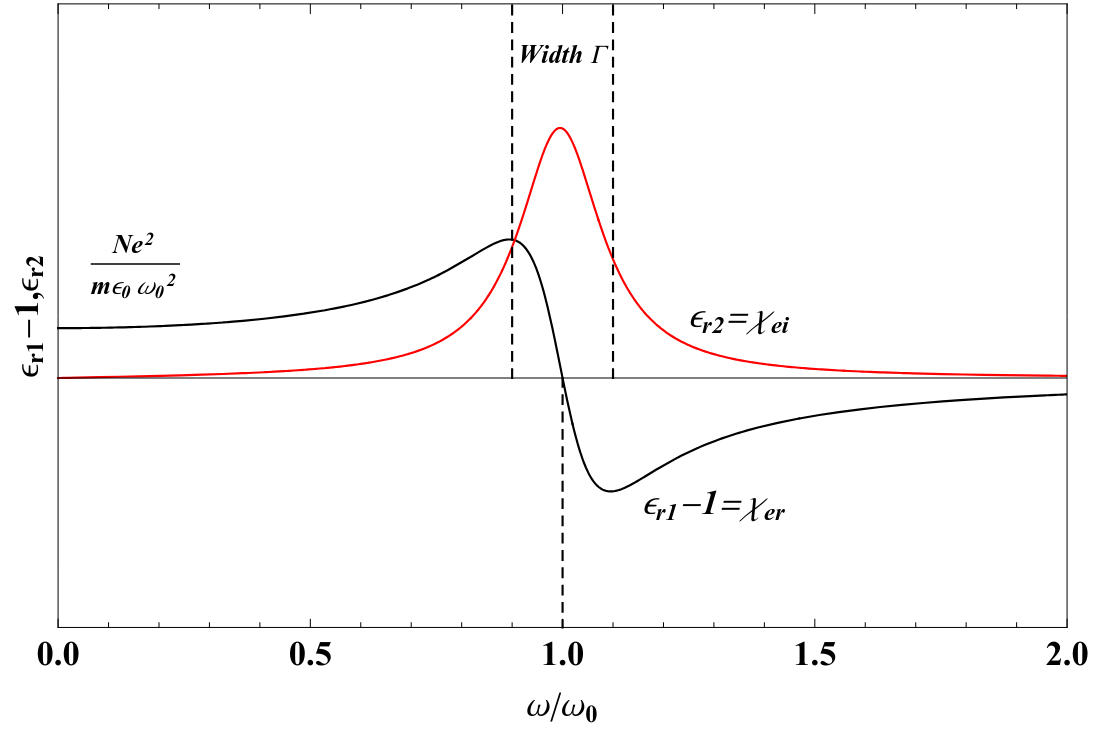
\includegraphics[width=0.5\textwidth]{realimg.png}
	\caption{The real and complex parts of permittivity for a a single resonant frequency $\omega_0$. In a dielectric there may be many such frequencies, which we label $\omega_j$.}
	\label{fig:gasses}
\end{figure}
In figure \ref{fig:gasses}, we visualise the real and imaginary parts of the refractive index for a given $\omega_0$. We describe observations below,
\begin{enumerate}
	\item $\omega = \omega_0$, refractive index is purely real, so we get maximum power transfer.
	\item $n_r > 1$, $\dv{n}{\omega} > 1$;
	\item $|\Gamma| < n_r$, $\dv{n}{\omega} < 1$;
	\item $n_r < 1$, $\dv{n}{\omega} > 0$;
	\begin{itemize}
		\item 1 and 3 are known as the \textit{normal dispersion regions} and 2 is known as the \textit{anomalous dispersion region}. 
	\end{itemize}
	
	\item In the limit $\omega \to 0$, we find,
	\begin{align}
		n_R \to 1 + \frac{q^2Nf_i}{2m\epsilon_0\omega_j^2} && n_I \to 0;
	\end{align}
	\item $n = c/v_p$, $v_p = \omega/k$, $n = ck/\omega$, and for some frequencies $n < 1$, in which case $\omega/k > c$
	\begin{itemize}
		\item However, $\dv{\omega}{k} < c$ always. 
	\end{itemize}
\end{enumerate}
\section{Waves in Conductors}
Metals and semiconductors have a lattice of fixed ions and electron gas, which are almost freely moving. Therefore, an external $\vb{E}$ field creates a current. We can the use Ohm's law $\vb{J} = \sigma \vb{E}$. We can rewrite the dispersion relation in equation \eqref{eq:dispersion} as,
\begin{equation}
	k_c = k_0\sqrt{\mu_r\epsilon_r}\sqrt{1 - i\frac{\sigma}{\epsilon_r \epsilon_0 \omega}} \label{eq:com}
\end{equation}
\subsection{Poor Conductors}
In poor conductors, we have that $\frac{\sigma}{\epsilon_r \epsilon_0\omega} <<1$, so we can perform a Taylor expansion on equation \eqref{eq:com},
\begin{equation}
	k_c \approx k_0 \sqrt{\mu_r\epsilon_r}(1 - \frac{i}{2}\frac{\sigma}{\epsilon_r \epsilon_0\omega}).
\end{equation}
Let us consider the modulus of the imaginary part of $k_c$,
\begin{equation}
	\abs{k_I} = \frac{\omega}{c}\sqrt{\mu_r\epsilon_r}\frac{\sigma}{2\epsilon_r \epsilon_0} = \frac{\sigma}{2}\sqrt{\frac{\mu_r\mu_0}{\epsilon_r\epsilon_0}}
\end{equation}
from which we can define the skin depth,
\begin{equation}
	\delta = \frac{1}{|k_I|} = 	\frac{2}{\sigma}\sqrt{\frac{\epsilon_r\epsilon_0}{\mu_r\mu_0}}.
\end{equation}
Let us recall the wavelength of light is given by,
\begin{equation}
	\lambda = \frac{2\pi}{\lambda} = \frac{2\pi c}{\omega}\frac{1}{\sqrt{\epsilon_r\mu_r}}.
\end{equation}
We are then interested in the ratio of the wavelength and skin depth, i.e., what fraction of the wavelength the wave can penetrate,
\begin{equation}
	\frac{\delta}{\lambda} = \frac{\omega}{\pi\sigma}\epsilon_r\epsilon_0
\end{equation}
and for a poor conductor, we find $\delta/\lambda << 1$. Therefore, an EM field can penetrate many wavelengths through a poor conductor before it decays.
\subsection{Good Conductors}
We now expect, $\frac{\sigma}{\omega\epsilon_o\epsilon_r} >> 1$. The dispersion relation \eqref{eq:dispersion} now reduces to,
\begin{equation}
	\begin{split}
	k_c & = \sqrt{\mu_r\epsilon_r}\sqrt{\frac{\omega\sigma}{\epsilon_r\epsilon_0}}\sqrt{\epsilon_0\mu_0}\underbrace{(-i)^{1/2}}_{\frac{1}{\sqrt{2}}(1-i)} \\
	& = \sqrt{\frac{\mu_r\mu_0\sigma\omega}{2}}(1-i)
\end{split}
\end{equation}
and thus,
\begin{align}
	\delta = \sqrt{\frac{2}{\mu_r\mu_0\sigma\omega}} &&\lambda = \frac{2\pi}{k_R} = 2\pi\delta
\end{align}
so,
\begin{equation}
	\frac{\sigma}{\lambda} = \frac{1}{2\pi} \sim 0.16
\end{equation}
so most of the wave is absorbed by a good conductor. Furthermore, if we calculate,
\begin{equation}
	\frac{B}{E} \sim \frac{k}{\omega} = \sqrt{\frac{\mu_r\mu_0\sigma}{\omega}}\underbrace{\frac{1}{\sqrt{2}}(1-i)}_{e^{-i\frac{\pi}{4}}}
\end{equation}
so the magnetic and electric field have a phase difference of $45^{\text{o}}$ in a conductor.
\section{Waves in Plasmas}
In a plasma, we have free electrons moving in the presence of stationary positive and neutral ions. We will consider the motion of the electrons in a plasma.
\subsection{The Drude Model}
We will consider the collisions in the plasma to be elastic. Since the electrons are also unbound, our equation of motion becomes,
\begin{equation}
	-e\vb{E} = m\dv[2]{\vb{x}}{t} = -k\vb{x}.
\end{equation}
We have that $\omega = \sqrt{k/m} \implies k = \omega^2m$, so,
\begin{equation}
	-e\vb{E} = -\omega^2m\vb{x} \implies \vb{x} = \frac{e}{m\omega^2}\vb{E}
\end{equation}
which is the electron displacement. Such a displacement causes a dipole moment,
\begin{equation}
	\vb{p} = - e\vb{x}
\end{equation}
and polarisation,
\begin{equation}
	\vb{P} = n\vb{p} = -\frac{Ne^2}{m\omega^2}\vb{E}
\end{equation}
from which we ca obtain our $\vb{D}$ field,
\begin{equation}
	\vb{D} = \epsilon_0\vb{E} + \vb{P} = \epsilon_0\left(1 - \frac{Ne^2}{m\omega^2\epsilon_0}\right)\vb{E}
\end{equation}
and thus we have found an equivalent $\epsilon_r$ for plasma. We can further define a \textit{plasma frequency},
\begin{equation}
	\omega_p^2 = \frac{Ne^2}{m\epsilon_0}
\end{equation}
so that,
\begin{equation}
	\vb{D} = \epsilon_0\left(1-\frac{\omega_p^2}{\omega^2}\right)\vb{E}.
\end{equation}
Collisions give rise to an average velocity of electrons, and this mechanism will cause a damping term in the equation of motion. If we consider $\gamma_c$ to be the collision frequency and $\tau_c = 1/\gamma_c$ to be the collision time, we can obtain a current by,
\begin{equation}
	\vb{J} = \omega_0 \vb{E} = -Ne\vb{v}_{\text{drift}}
\end{equation}
where we can define,
\begin{align}
	\vb{v}_{\text{drift}} = -\frac{e\vb{E}}{m}\frac{1}{\gamma_c} && \sigma_0 = \frac{Ne^2}{m}\frac{1}{\gamma_c} = \frac{\epsilon_0\omega_p^2}{\gamma_c}.
\end{align}
\subsection{Drude Model with Collisions}
Let us now consider inelastic collisions in a plasma. We add a damping term $\beta$ to our equation of motion,
\begin{equation}
	m\Ddot{\vb{x}} + m\beta\Dot{\vb{x}} = -e\vb{E}_0e^{i\omega t}
\end{equation}
from which we obtain a displacement,
\begin{equation}
	\vb{x} = \frac{-\frac{e}{m}}{-\omega^2 + i\omega\beta}\vb{E}_0e^{i\omega t}
\end{equation}
and velocity,
\begin{equation}
	\Dot{x} = \frac{-ie\frac{\omega}{m}}{-\omega^2 + i\omega\beta}\vb{E}_0e^{i\omega t}
\end{equation}
We will then have a current,
\begin{equation}
	\vb{J} = \sigma(\omega)\vb{E} = -Ne\Dot{x}
\end{equation}
such that,
\begin{equation}
	\sigma(\omega) = \frac{\sigma_0}{1 + i\frac{\omega}{\gamma_c}}
\end{equation}
where we define the DC conductivity,
\begin{equation}
	\sigma_0 = \frac{Ne^2}{m}\frac{1}{\gamma_c}.
\end{equation}
Let us investigate the permittivity. Using $\vb{P}  = N(-e)\vb{x}$ from the Drude model, we find,
\begin{equation}
	\chi_E = \frac{Ne^2}{\epsilon_0m}\frac{1}{-\omega^2 + i\gamma_c\omega}
\end{equation}
and $\epsilon_r = 1 + \chi_E$ so,
\begin{equation}
	\epsilon_r = 1+ \frac{\omega_p^2}{-\omega^2 + i\gamma_c\omega}. \label{eq:perm}
\end{equation}
\subsubsection{Low frequency waves in plasma}
If we consider $\omega << \gamma_c$, we reduce equation \eqref{eq:perm} to,
\begin{equation}
	\epsilon_r = 1+ \frac{\sigma_0}{i\omega\epsilon_0} \simeq -i\frac{\sigma_0}{\omega\epsilon_0}.
\end{equation}
The refractive index is then,
\begin{equation}
	n = \sqrt{\epsilon_r} = \sqrt{\frac{\sigma_0}{\omega\epsilon_0}}\sqrt{-i} = \sqrt{\frac{\sigma_0}{2\omega\epsilon_0}}(1-i)
\end{equation}
so we find $n_R = n_I$. We then find the skin depth to be,
\begin{equation}
	\sigma = \sqrt{\frac{2}{\mu_0\sigma_0\omega}}.
\end{equation}
\subsubsection{High frequency waves in plasma}
For a high frequency wave, $\omega >> \gamma_c$, we find,
\begin{equation}
	\epsilon_r \simeq 1 - \frac{\omega_p^2}{\omega^2}.
\end{equation}
We can then extract the dispersion relation for a plasma,
\begin{align}
	\omega^2 = k^2c^2 + \omega_p^2\\
	k = \pm\frac{1}{c}\left(\omega^2 + \omega_p^2\right)^{\frac{1}{2}}
\end{align}
we then find that $\epsilon_r$ is real no matter the value of $\omega$, EM waves travel through plasmas as if through vacuum. Let us consider some limiting situations with frequency,
\begin{enumerate}
	\item $\omega = \omega_p \implies k = 0$, and we find, $k \to 0 \implies v_p \to \infty$ and $v_g \to 0$, so the wave ceases to propagate.
	\item $\omega >> \omega_p$
	\item $\omega << \omega_p$, we find that $k$ is purely imaginary and described by,
	\begin{equation}
		kc = -i\sqrt{\omega_p^2 -\omega^2}
	\end{equation}
	and the electromagnetic wave undergoes an exponential decay.
\end{enumerate}
\chapter{Reflection and Refraction}
\section{Maxwell's Equations and Boundary Conditions}
We will consider the boundary conditions for $\vb{H}, \vb{B}, \vb{E},$ and $\vb{D}$  by Maxwell's equations.
\subsection{Transverse Component of Electric Field}
\begin{figure}[h]
	\centering
	\begin{tikzpicture}[scale=1.5]
		\draw (0,0) -- (5,0);
		\fill[pattern={Lines[angle = 45, distance=0.1cm]}] (0,0) rectangle (5, -0.1);
		\draw[-latex] (1,2) -- (2.5,0) node[anchor=south west] {$\vb{E}_1$};
		\draw[-latex, dashed] (1, 2) -- (1,0) node[anchor=south west] {$\vb{E}_{1\parallel}$};
		\draw[-latex, dashed] (1,2) -- (2.5,2) node[anchor=west] {$\vb{E}_{1\perp}$};
		\draw[-latex, color=blue] (2.5,0) -- (3, -1.5) node[anchor = north west] {$\vb{E}_2$};
		\draw[-latex, color=blue, dashed] (2.75,-0.75) -- (2.75, -1.5) node[anchor = north] {$\vb{E}_{2\parallel}$};
		\draw[-latex, color=blue, dashed] (2.75,-0.75) -- (3,-0.75) node[anchor = west] {$\vb{E}_{2\perp}$};
		\begin{scope}[thick, dashed, color = red, decoration={
				markings,
				mark=at position 0.5 with {\arrow{>}}}
			] 
		\draw[postaction={decorate}] (0.75,-1) -- (4.25,-1);
		\draw[postaction={decorate}]  (4.25,-1) -- (4.25,1) node[anchor=south west] {$C$};
		\draw[postaction={decorate}]	 (4.25,1) -- (0.75, 1);
		\draw[postaction={decorate}]	 (0.75, 1)-- (0.75, -1);
		\end{scope}
		\node[anchor=south west] at (0,0) {$\epsilon_1,\mu_1$};
		\node[anchor=north west] at (0,-0.1) {$\epsilon_2,\mu_2$};
		\draw[thick, decoration={brace,mirror,raise=5pt},decorate] (4.25,-1) -- (4.25,1) node[midway, right=6pt, anchor = south west] {$\Delta H$};
		\draw[thick, decoration={brace,mirror,raise=5pt},decorate] (4.25,1)--(0.75,1) node[midway, above=6pt] {$\Delta W$};
	\end{tikzpicture}
	\caption{}
	\label{fig:trans E}
\end{figure}
Let us consider a setup as in figure \ref{fig:trans E}, where an electric field is travelling through a material with $\epsilon = \epsilon_1$ and $\mu = \mu_1$ incident on the surface of a material with $\epsilon = \epsilon_2$ and $\mu = \mu_2$. Let us consider Ampere's law over a loop $C$ with width $\Delta W$ and height $\Delta H$,
\begin{equation}
	\oint_C \vb{E}\cdot\dd\vb{l} = -\pdv{t}\oint\vb{B}\cdot\dd\vb{S}
\end{equation}
\appendix
\chapter{Revision Equations}

\section{Potentials}
\begin{tcolorbox}[colback=red!5!white,colframe=red!75!black,title=Static Electric Potential]
	\begin{align}
		\vb{E} &= - \grad \phi \\
		\laplacian{\phi} &= - \frac{\rho}{\varepsilon_0}
	\end{align}
\end{tcolorbox}
\begin{tcolorbox}[colback=blue!5!white,colframe=blue!75!black,title=Static Magnetic Potential]
	\begin{align}
		\vb{B} &= \curl{\vb{A}} \\
		-\curl{\vb{B}} &= \laplacian{\vb{A}} = - \mu_0 \vb{J}
	\end{align} 
	if we choose,
	\begin{align}
		\vb{A} \to \vb{A} + \grad{\psi} && \div{\vb{A}} = 0.
	\end{align}
\end{tcolorbox}
\begin{tcolorbox}[colback=green!5!white,colframe=green!75!black,title=Dynamic Potentials]
	\begin{align}
		\laplacian\vb{A} - \mu_0\varepsilon_0 \pdv{\vb{A}}{t} &= - \mu_0 \vb{J} \label{eq:A} \\
		\laplacian\vb{\phi} - \mu_0\varepsilon_0\pdv{\phi}{t} &= -\frac{\rho}{\varepsilon_0} \label{eq:phi}
	\end{align}
\end{tcolorbox}
\section{Gauges}
\begin{tcolorbox}[colback=red!5!white,colframe=red!75!black,title=Coloumb Gauge]
	\begin{equation}
		\div{\vb{A}} = 0
	\end{equation}
\end{tcolorbox}
\begin{tcolorbox}[colback=blue!5!white,colframe=blue!75!black,title=Lorenz Gauge]
	\begin{equation}
		\div{\vb{A}} + \frac{1}{c^2}\pdv{\phi}{t} = 0
	\end{equation}
\end{tcolorbox}
\section{Vector Identities}
\begin{tcolorbox}[colback=blue!5!white,colframe=blue!75!black,title=Laplacian of a Vector]
	\begin{equation}
		\curl{\curl{\vb{A}}} = \grad\left(\div{\vb{A}}\right) - \laplacian{\vb{A}}
	\end{equation}
\end{tcolorbox}
\section{EM Waves}
\begin{tcolorbox}[colback=red!5!white,colframe=red!75!black,title=Relation between $\vb{E}$ and $\vb{B}$]
	\begin{equation}
		\vb{B} = \frac{1}{c}\hat{\vb{k}}\cross \vb{E}. \label{eq:A4}
	\end{equation}
\end{tcolorbox}

\end{document}
